\documentclass[12pt,a4paper]{article}

\title{LISTA 5 - ELM}

\centering

\author{Andre Werneck - MATRICULA : 2017088140}

\usepackage{Sweave}
\usepackage{graphics}

\begin{document}

\maketitle

\begin{center}

REDES NEURAIS ARTIFICIAIS

\end{center}

\Sconcordance{concordance:exELM.tex:exELM.Rnw:%
1 27 1 1 53 5 1 1 10 1 22 2 1 1 42 2 1 1 4 1 2 6 1 2 2 6 1 1 42 2 1 1 4 %
1 2 6 1 2 2 8 1}


\newpage

\section{Exercicio 1 - Plot da Superficie de Separacao}



\begin{itemize}

\item Base "2dnormals"
\newline



ELM com p=5 neuronios


\begin{figure}[!htb]
\begin{center}
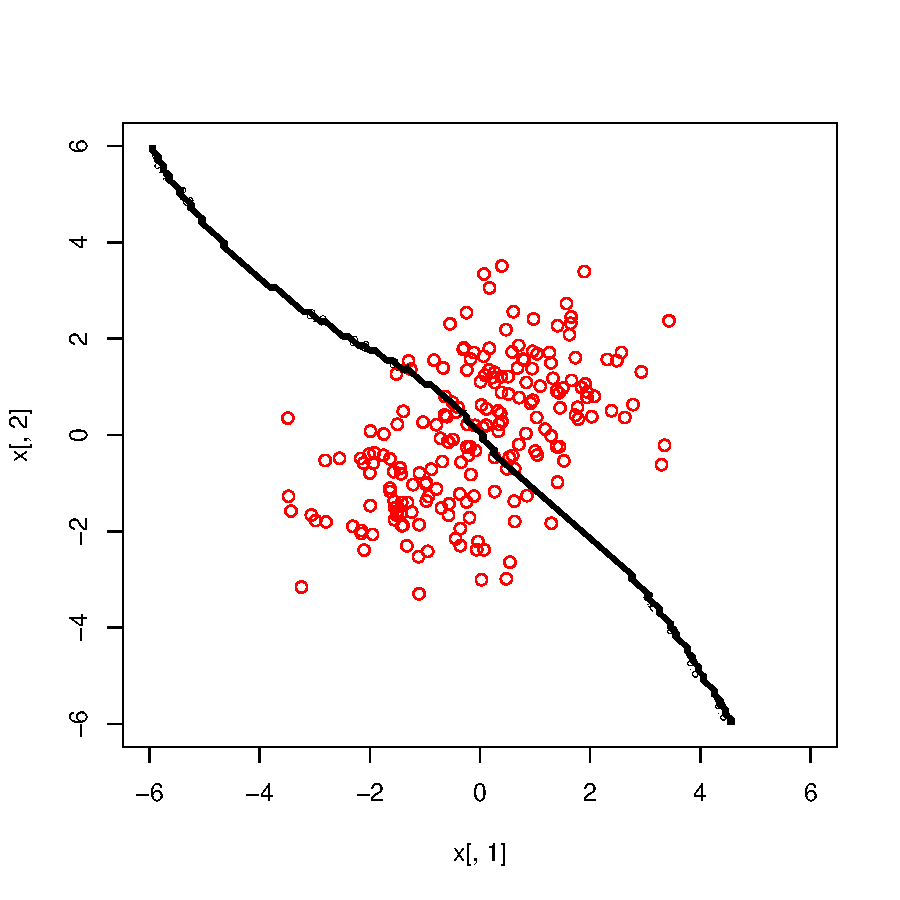
\includegraphics{exELM-005}
\end{center}
\caption{Contorno da Superficie em 2D}
\label{Contorno da Superficie em 2D}
\end{figure}

\begin{figure}[!htb]
\begin{center}
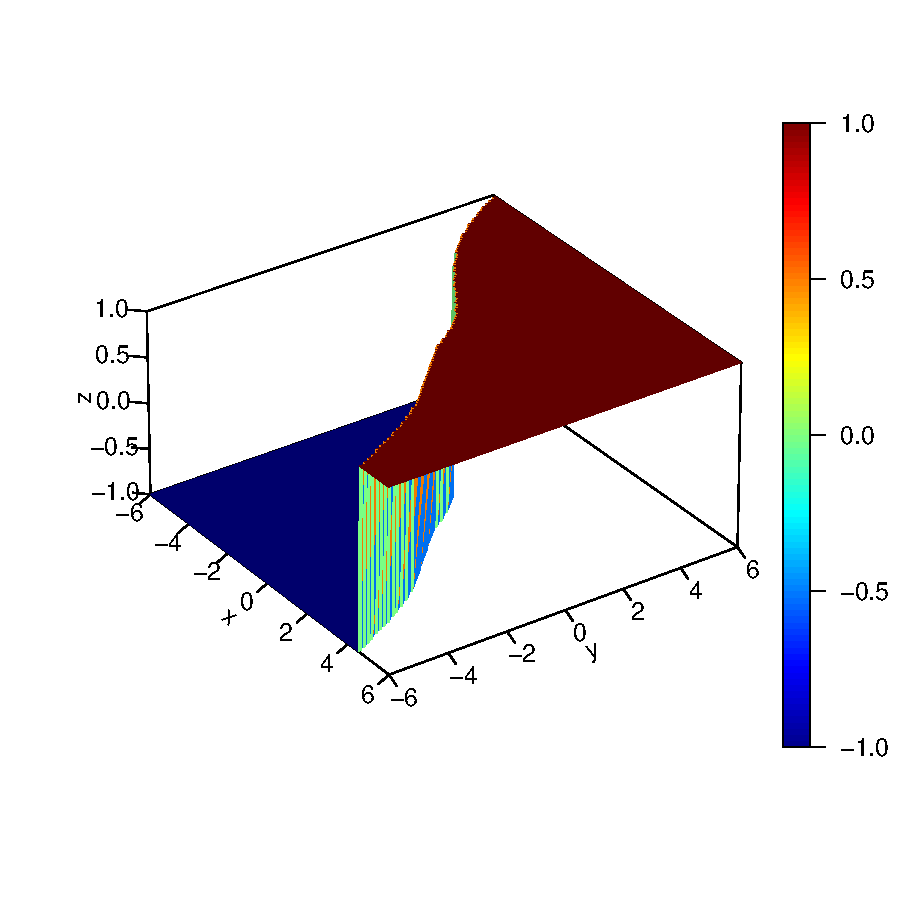
\includegraphics{exELM-006}
\end{center}
\caption{Contorno da Superficie em 3D}
\label{Contorno da Superficie em 3D}
\end{figure}

ELM com p=20 neuronios


\begin{figure}[!htb]
\begin{center}
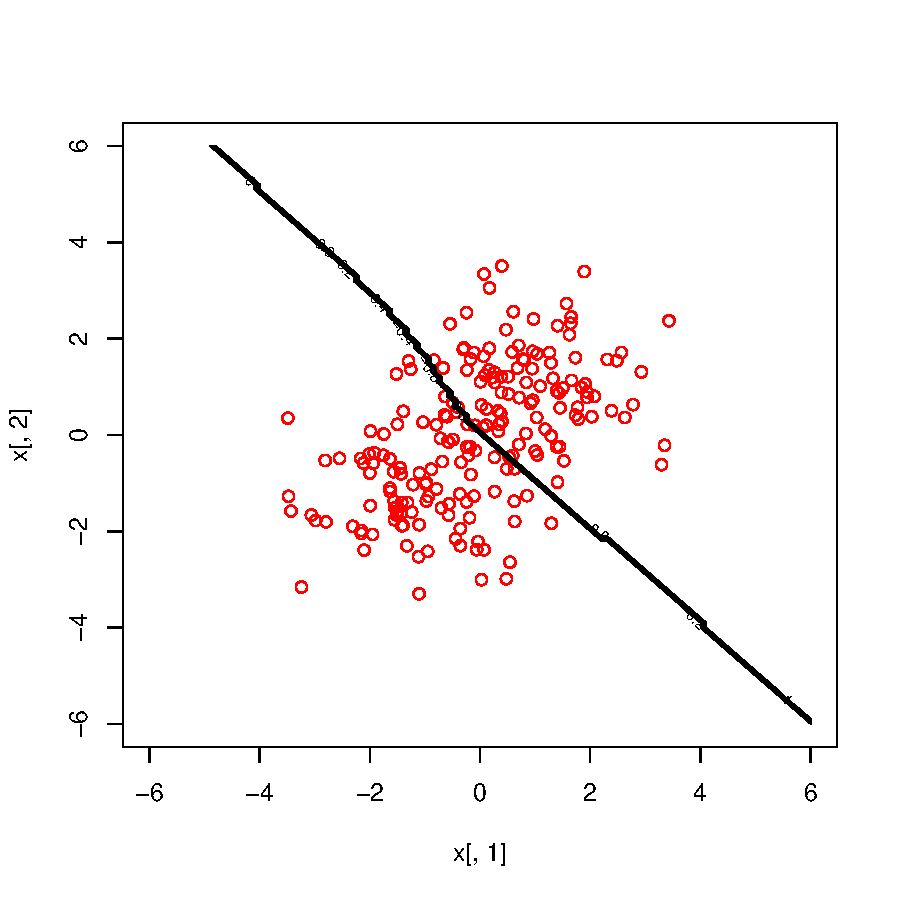
\includegraphics{exELM-008}
\end{center}
\caption{Contorno da Superficie em 2D}
\label{Contorno da Superficie em 2D}
\end{figure}

\begin{figure}[!htb]
\begin{center}
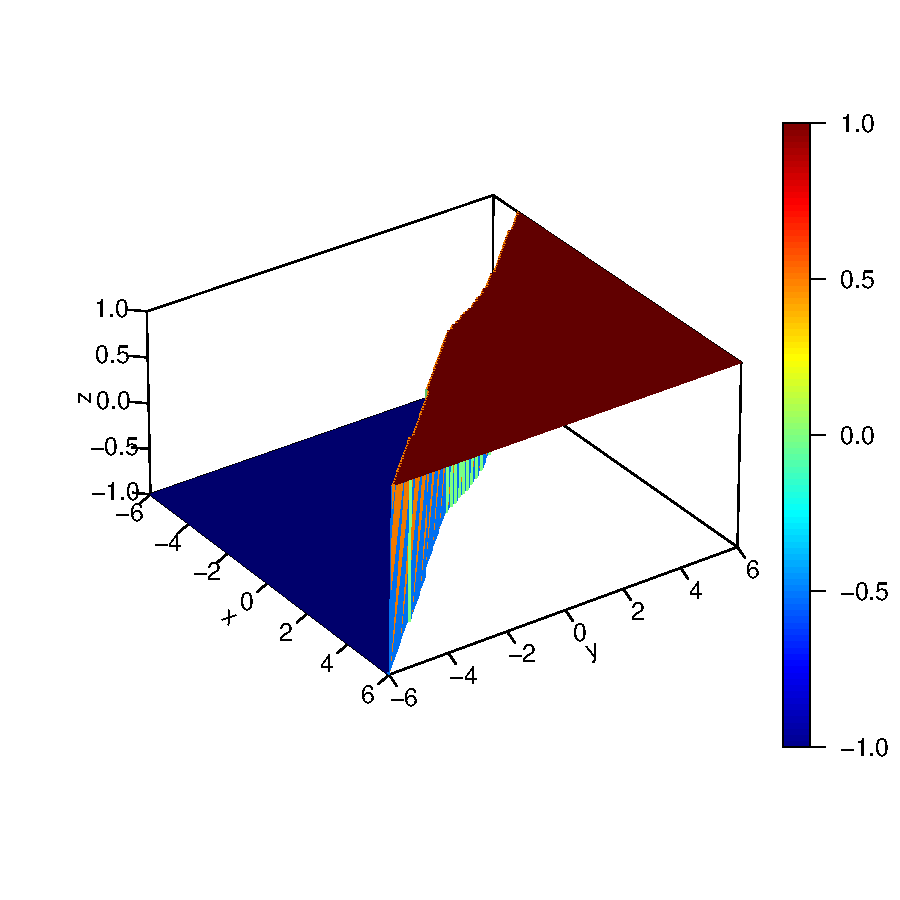
\includegraphics{exELM-009}
\end{center}
\caption{Contorno da Superficie em 3D}
\label{Contorno da Superficie em 3D}
\end{figure}


\end{itemize}

\end{document}
